% This is samplepaper.tex, a sample chapter demonstrating the
% LLNCS macro package for Springer Computer Science proceedings;
% Version 2.21 of 2022/01/12
%
\documentclass[runningheads]{llncs}
%
\usepackage[utf8]{inputenc}
\usepackage[T1]{fontenc}
\usepackage{amsmath}
% T1 fonts will be used to generate the final print and online PDFs,
% so please use T1 fonts in your manuscript whenever possible.
% Other font encondings may result in incorrect characters.
%
\usepackage{graphicx}
% Used for displaying a sample figure. If possible, figure files should
% be included in EPS format.
\usepackage{subcaption}
\usepackage{float}
%
% If you use the hyperref package, please uncomment the following two lines
% to display URLs in blue roman font according to Springer's eBook style:
%\usepackage{color}
%\renewcommand\UrlFont{\color{blue}\rmfamily}
%\urlstyle{rm}
%
\begin{document}
%
\title{Classificação de Imagens ERCP com Redes Neurais Convolucionais Profundas}
%
\titlerunning{Classificação de Imagens ERCP com CNNs}
% If the paper title is too long for the running head, you can set
% an abbreviated paper title here
%
\author{
Carlos da Mota Bergueira (pg11605@alunos.uminho.pt) \\
Diego Jefferson Mendes Silva (pg59999@alunos.uminho.pt) \\
Filipa Araújo Pereira (pg42201@alunos.uminho.pt) \\
Rui Manuel Martins Marques Rodrigues (pg7942@alunos.uminho.pt)
}
%
\authorrunning{C. Bergueira, D. Silva, F. Pereira, R. Rodrigues}
% First names are abbreviated in the running head.
% If there are more than two authors, 'et al.' is used.
%
\institute{Universidade do Minho, Braga, Portugal \\
% \email{pg11605@alunos.uminho.pt, pg59999@alunos.uminho.pt, pg42201@alunos.uminho.pt, pg7942@alunos.uminho.pt}
}
%
\maketitle              % typeset the header of the contribution
%
\begin{abstract}
Este relatório apresenta um estudo comparativo de quatro arquiteturas CNN
pré-treinadas para classificação multiclasse de imagens de ERCP:
DenseNet121, ResNet50, MobileNetV2 e EfficientNet-B7. O objetivo principal
foi maximizar o F1-score macro num cenário com forte desequilíbrio de
classes, com predominância de Lithiasis e sub-representação de Biliary Leaks.
Foram avaliadas mais de 20 variantes experimentais, combinando transfer
learning, funções de perda ponderadas, técnicas de regularização e estratégias
de inferência robusta. Os resultados mostram que a DenseNet121 obteve o
melhor desempenho global (F1 macro = 0.7076; accuracy = 0.7266), seguida da
ResNet50 (0.6647; 0.7041). EfficientNet-B7 e MobileNetV2 apresentaram
desempenhos inferiores (\(\approx\)0.555), associados a sobreajuste e menor
capacidade de adaptação, respetivamente. A análise por classe confirma que o
tratamento explícito do desequilíbrio (Focal Loss, class weights, Mixup e TTA)
teve impacto superior ao de ajustes isolados de pré-processamento. Os
resultados reforçam a adequação de abordagens orientadas a classes minoritárias
em tarefas médicas de risco elevado e apontam o ensemble como via promissora
de melhoria.

\keywords{CNN \and transfer learning \and ERCP \and F1 macro \and desequilíbrio de classes \and ensemble}
\end{abstract}
%
\section{Introdução}

\subsection{Problema e Dataset}
O dataset MIQR-CC~\cite{martins2025} consiste em imagens de ERCP classificadas em quatro
categorias clínicas: Biliary Leaks, Lithiasis, Normal e Stricture. A
distribuição é fortemente desequilibrada, com predominância de Lithiasis e
sub-representação de Biliary Leaks.

\begin{table}[ht]
\caption{Distribuição das classes por split.}
\label{tab:dataset_split}
\centering
\begin{tabular}{lccccc}
\hline
Split & Total & Biliary Leaks & Lithiasis & Normal & Stricture \\
\hline
Treino & 1067 & 110 (10.3\%) & 505 (47.3\%) & 197 (18.5\%) & 255 (23.9\%) \\
Validação & 234 & 24 & 98 & 59 & 53 \\
Teste & 267 & 17 & 123 & 43 & 84 \\
\hline
\end{tabular}
\end{table}

A métrica principal é o F1-score macro:
\begin{equation}
F_1^{\text{macro}} = \frac{1}{C}\sum_{c=1}^{C} \frac{2 P_c R_c}{P_c + R_c}
\end{equation}

Esta métrica penaliza fortemente modelos que ignoram classes minoritárias,
mesmo quando a accuracy global é elevada.

\subsection{Motivação para Transfer Learning}
Todos os modelos foram inicializados com pesos ImageNet. Dado o tamanho do
conjunto de treino (1067 imagens), o treino de raiz seria instável e propenso
a sobreajuste. O transfer learning fornece descritores visuais genéricos que
aceleram convergência e reduzem a necessidade de dados anotados~\cite{tajbakhsh2016}.

\section{Arquiteturas Estudadas}

\subsection{DenseNet121}
Na DenseNet, cada camada recebe a concatenação das ativações anteriores:
\begin{equation}
\mathbf{x}_L = H_L([\mathbf{x}_0, \mathbf{x}_1, \ldots, \mathbf{x}_{L-1}])
\end{equation}
Esta conectividade densa favorece reutilização de características de baixo
nível e propagação de gradiente robusta~\cite{huang2017}.

\subsection{ResNet50}
A ResNet aprende funções residuais:
\begin{equation}
\mathbf{x}_{L+1} = \mathcal{F}(\mathbf{x}_L, \{W_i\}) + \mathbf{x}_L
\end{equation}
As conexões de atalho mitigam vanishing gradients e estabilizam o treino em
redes profundas~\cite{he2016}.

\subsection{MobileNetV2}
A MobileNetV2 usa blocos inverted residual com convoluções depthwise separable,
reduzindo custo computacional de
\(O(D_k^2MN)\) para \(O(D_k^2M + MN)\), com menor capacidade representacional
face a arquiteturas maiores~\cite{sandler2018}.

\subsection{EfficientNet-B7}
A EfficientNet aplica compound scaling conjunto de profundidade, largura e
resolução:
\begin{equation}
d = \alpha^{\phi}, \quad w = \beta^{\phi}, \quad r = \gamma^{\phi}
\end{equation}
Embora muito expressiva, a variante B7 é sensível a batch size e ao regime de
fine-tuning parcial~\cite{tan2019}.

\section{Progressão Experimental por Arquitetura}

\subsection{DenseNet121}
Foram avaliadas sete versões. O salto principal ocorreu após a introdução
explícita de técnicas orientadas a classes minoritárias
(Focal Loss + CE ponderada, Mixup, TTA e threshold tuning), elevando o F1 macro
de 0.545 para 0.647. A adição de CLAHE offline e resolução 256\(\times\)256
(v100) representou um ganho adicional de 6.1\,pp, culminando em
F1 macro 0.7076 e accuracy 0.7266 no conjunto de teste.

\begin{figure}[H]
  \centering
  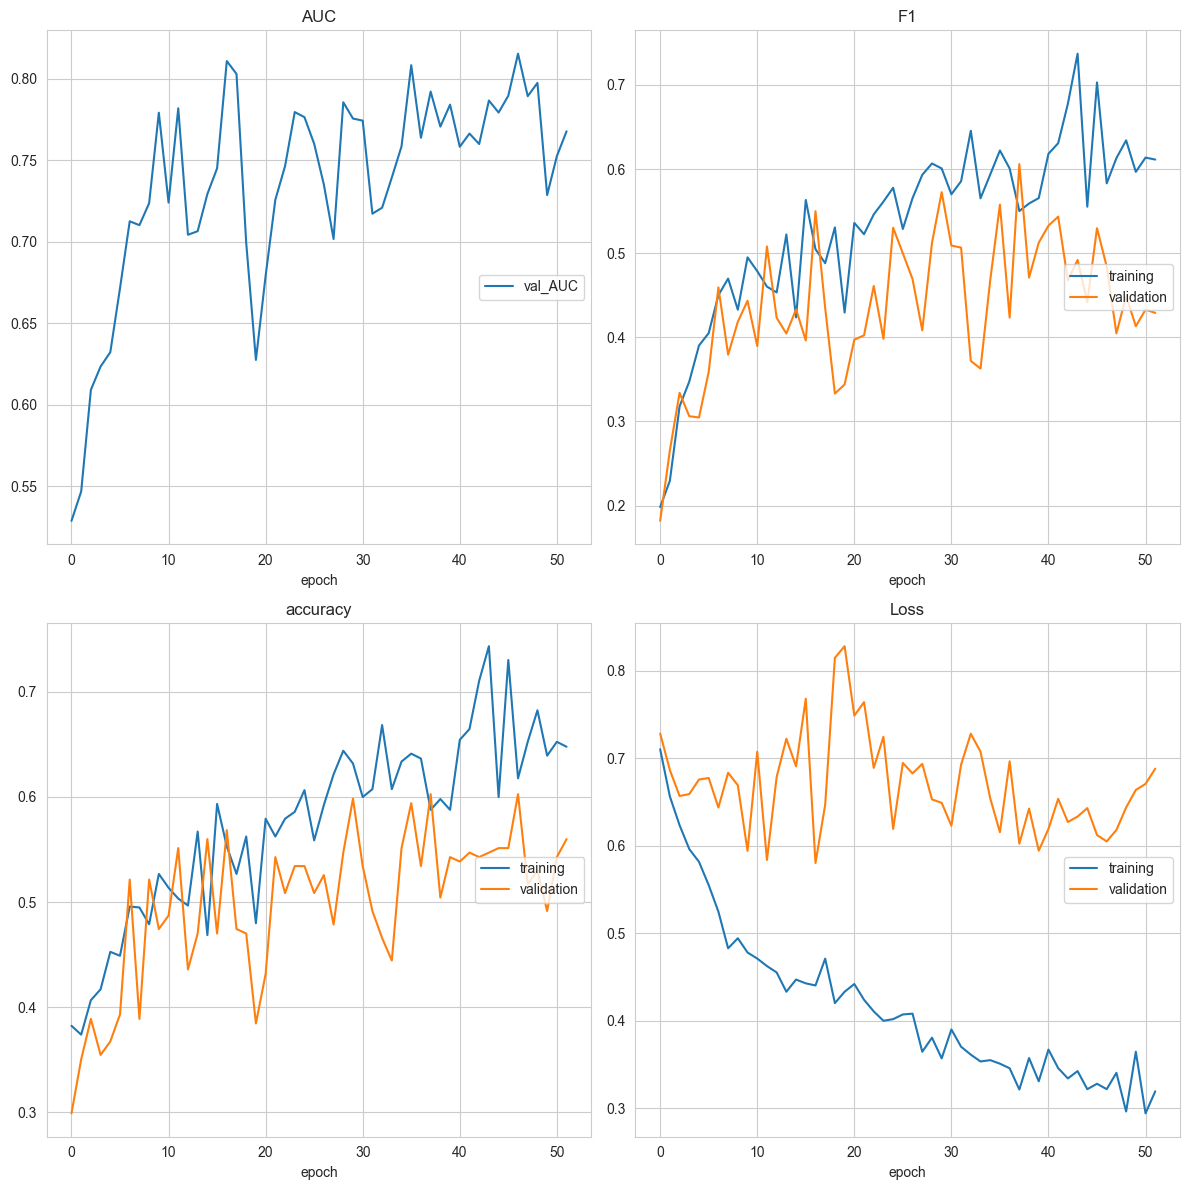
\includegraphics[width=0.95\textwidth]{images/treino-densenet.png}
  \caption{Curvas de treino da DenseNet121 (melhor configuração, v100):
    F1-score macro e função de perda em treino e validação ao longo das épocas.}
  \label{fig:treino_densenet}
\end{figure}

A Figura~\ref{fig:treino_densenet} revela um padrão de convergência estável e
progressivo. O F1 de treino sobe monotonicamente de~\(\approx\)0.17 para
\(\approx\)0.63 ao longo de 46 épocas, enquanto o F1 de validação acompanha
com um desfasamento moderado, atingindo \(\approx\)0.51 e estabilizando a
partir da época~30. A perda de treino decresce de forma contínua
(\(\approx\)1.37\(\rightarrow\)0.82) e a perda de validação apresenta apenas
uma ligeira subida residual (\(\approx\)1.38\(\rightarrow\)1.28), sem
divergência --- indicador de ausência de sobreajuste severo. O diferencial
treino-validação em F1 (\(\approx\)0.12) é consistente com o nível de
regularização aplicado (Mixup \(\alpha\!=\!0.4\), Dropout, label smoothing) e
com o tamanho do conjunto de treino. O salto observado no F1 de validação final
face ao valor durante o treino (\(\approx\)0.51\(\rightarrow\)0.71) deve-se ao
TTA e ao threshold tuning aplicados apenas na fase de avaliação, confirmando a
importância destas técnicas de inferência robusta.

\subsection{ResNet50}
Quatro versões foram comparadas. A melhor configuração introduziu CLAHE offline,
pré-processamento guiado pelo domínio (ROI circular, ScaleIntensityRangePercentiles),
Dropout(0.3) no classificador e data augmentation conservadora, atingindo
F1 macro 0.6647 e accuracy 0.7041 no conjunto de teste.

\begin{figure}[H]
  \centering
  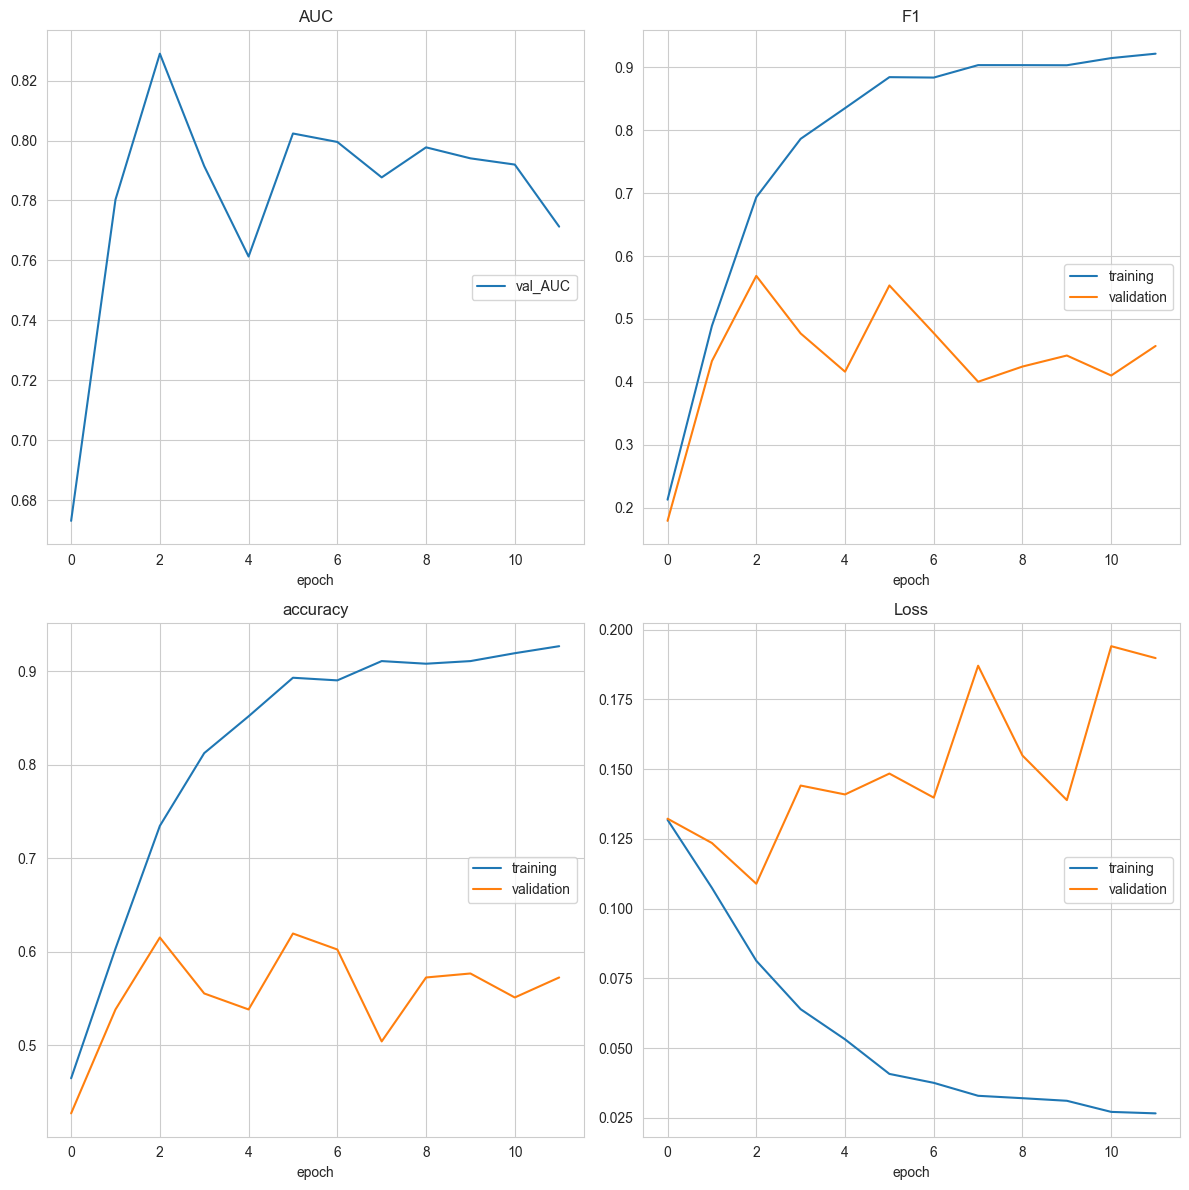
\includegraphics[width=0.95\textwidth]{images/treino-resnet.png}
  \caption{Curvas de treino da ResNet50 (melhor configuração): AUC-ROC de
    validação, F1-score macro, accuracy e função de perda ao longo das épocas.}
  \label{fig:treino_resnet}
\end{figure}

A Figura~\ref{fig:treino_resnet} mostra um padrão oscilatório ao longo de
50~épocas, característico do scheduler CosineAnnealingLR em presença de
desequilíbrio de classes. O AUC de validação sobe de \(\approx\)0.55 para
\(\approx\)0.80 com crescimento mais marcado até à época~20, depois
estabilizando com oscilações de \(\pm\)0.05. O F1 de treino sobe
gradualmente de \(\approx\)0.21 para \(\approx\)0.62, enquanto o F1 de
validação oscila entre 0.35 e 0.65, terminando em \(\approx\)0.62. Esta
variância elevada na validação reflete a sensibilidade da métrica macro ao
comportamento nas classes minoritárias: pequenas variações na fronteira de
decisão de Biliary Leaks produzem saltos amplos no F1 macro. A perda de
treino decresce de forma regular (\(\approx\)0.8\(\rightarrow\)0.32) ao
passo que a perda de validação oscila sem tendência de divergência clara,
confirmando a adequação do Dropout como regularizador. A accuracy de
validação (\(\approx\)0.55--0.60) ficou abaixo da de treino
(\(\approx\)0.65--0.73), desfasamento esperado num cenário com distribuição
de classes diferente entre splits.

\subsection{MobileNetV2}
O desempenho variou entre 0.306 e 0.556. O melhor resultado foi obtido com
CLAHE offline, imagens RGB com normalização ImageNet e learning rates
diferenciados por grupo de camadas, alcançando F1 macro 0.5558 e accuracy
0.6629 no conjunto de teste.

\begin{figure}[H]
  \centering
  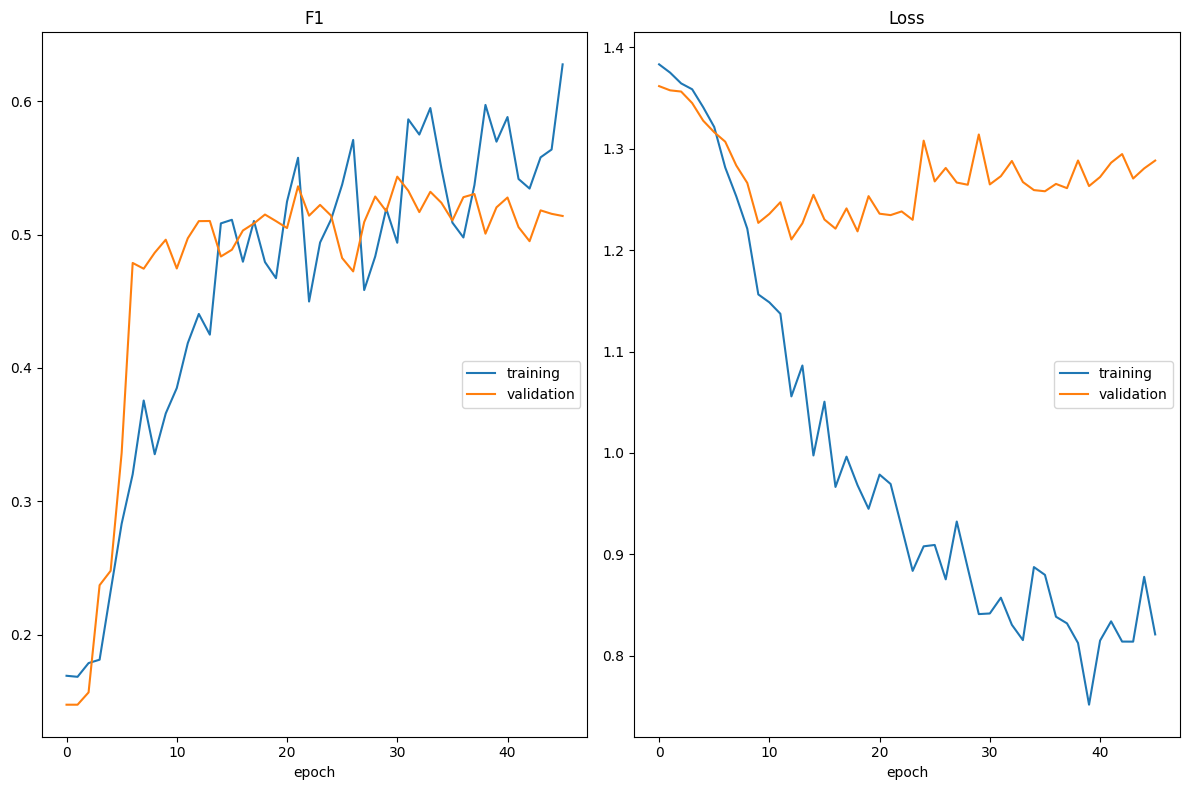
\includegraphics[width=0.95\textwidth]{images/treino-mobilenet.png}
  \caption{Curvas de treino da MobileNetV2: sobreajuste severo após
    desbloqueio do backbone na fase~2 de fine-tuning.}
  \label{fig:treino_mobilenet}
\end{figure}

A Figura~\ref{fig:treino_mobilenet} ilustra o fenómeno de sobreajuste
catastrófico observado nas variantes com fine-tuning faseado. Após
aproximadamente 10~épocas com o backbone congelado (fase~1), o desbloqueio
da totalidade dos pesos (fase~2) provocou memorização rápida do conjunto de
treino: o F1 de treino convergiu para \(\approx\)1.0 e a accuracy de treino
para~1.0 em cerca de 15~épocas, enquanto o F1 de validação estabilizou em
\(\approx\)0.40--0.50 e a perda de validação divergiu explosivamente para
\(\approx\)5.0. Este padrão evidencia que a MobileNetV2, com capacidade
representacional mais limitada que as restantes arquiteturas, é incapaz de
generalizar sob esta estratégia de fine-tuning: a transição abrupta de
backbone congelado para completamente desbloqueado, sem warm-up adequado,
causa atualização incontrolada dos pesos em camadas que já tinham aprendido
características genéricas do ImageNet. A solução adoptada nas versões v6/v7
--- differential learning rates sem fase de congelamento --- visou precisamente
mitigar este comportamento.

\subsection{EfficientNet-B7}
A melhor versão (RR12) obteve F1 macro 0.5557 e accuracy 0.6217 no conjunto
de teste, com congelamento de BatchNorm e fine-tuning parcial dos últimos
blocos. O padrão dominante nas variantes iniciais foi sobreajuste precoce.

\begin{figure}[H]
  \centering
  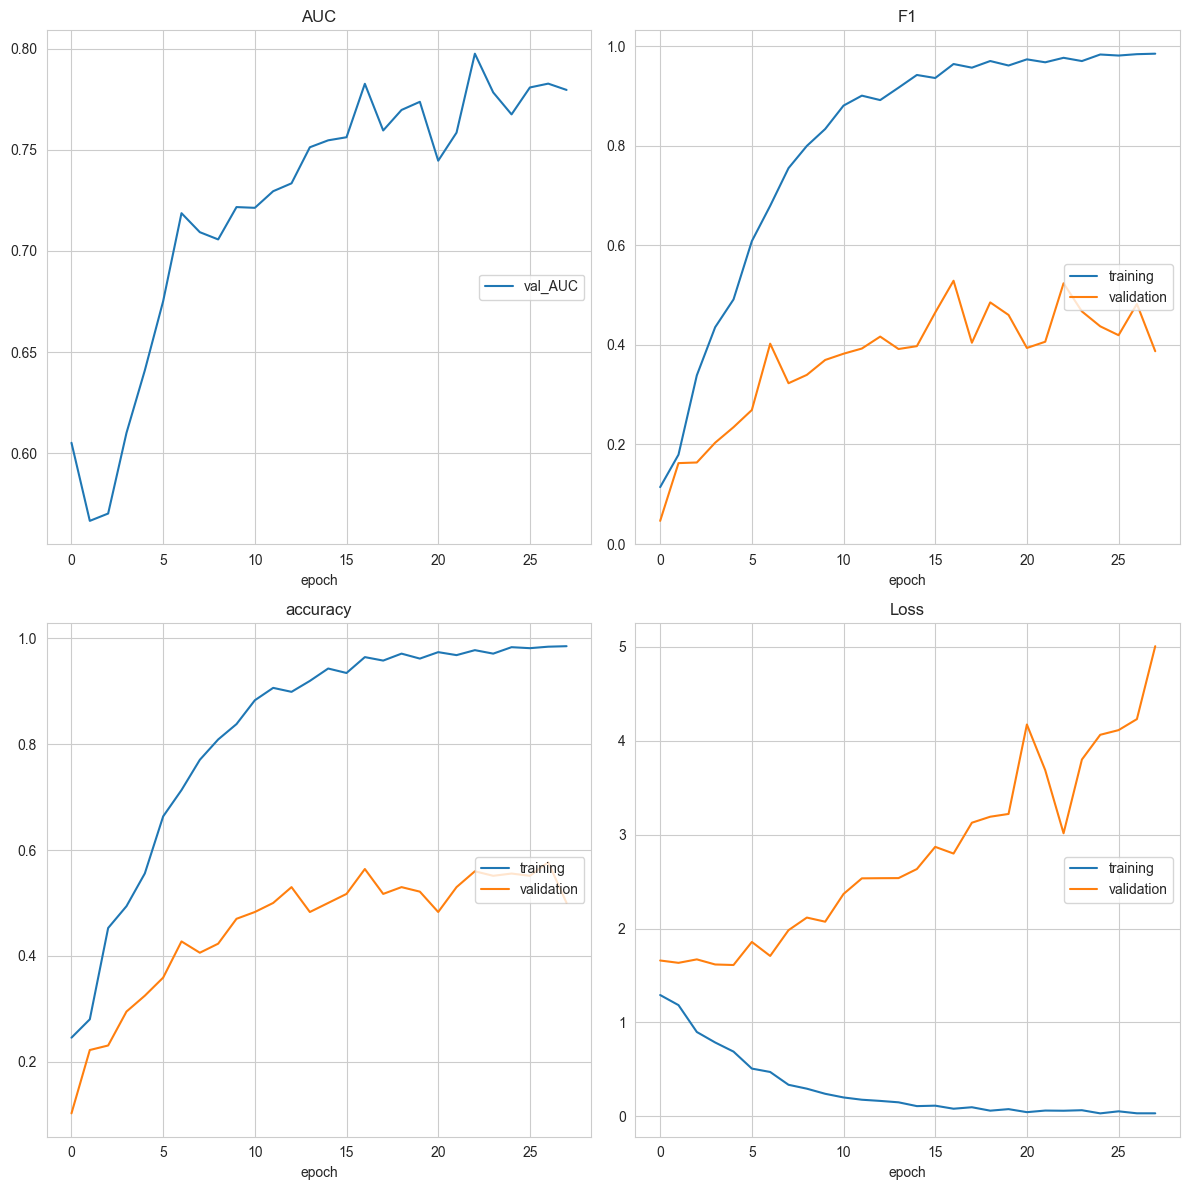
\includegraphics[width=0.95\textwidth]{images/treino-efficientnet.png}
  \caption{Curvas de treino da EfficientNet-B7: rápida memorização do
    conjunto de treino com degradação simultânea da validação.}
  \label{fig:treino_efficientnet}
\end{figure}

A Figura~\ref{fig:treino_efficientnet} documenta o comportamento de
sobreajuste precoce da EfficientNet-B7. O F1 de treino atinge
\(\approx\)0.90 e a accuracy de treino \(\approx\)0.93 em apenas 3--4~épocas,
enquanto o AUC de validação sobe rapidamente para \(\approx\)0.82 na
época~2 e depois recua para \(\approx\)0.76. O F1 de validação atinge um
máximo de \(\approx\)0.55 na época~2 e regride para \(\approx\)0.45, e a
perda de validação aumenta de \(\approx\)0.125 para \(\approx\)0.190 à
medida que a perda de treino colapsa para \(\approx\)0.025. O early stopping
interrompeu o treino na época~11, limitando a degradação mas também o espaço
de exploração. Esta dinâmica é consequência da elevada capacidade do
EfficientNet-B7 (\(\approx\)66M parâmetros): a rede memoriza as 1067 imagens
de treino em poucos passos de gradiente, não havendo regularização suficiente
para forçar a aprendizagem de representações generalizáveis. A elevação do
AUC para 0.87 no teste final --- acima do F1 macro --- indica que o modelo
preserva alguma capacidade discriminativa probabilística, aproveitada
parcialmente pelo TTA de 8 passes na avaliação final.

\section{Comparativo Detalhado}

\subsection{Configuração dos Melhores Modelos}
Para garantir reprodutibilidade, todos os modelos fixaram a semente aleatória em~42
(\texttt{torch.manual\_seed}, \texttt{numpy.random.seed} e \texttt{random.seed}),
e o código completo está disponível no repositório do grupo.

\begin{table}[ht]
\caption{Resumo das melhores configurações por arquitetura.}
\label{tab:best_configs}
\centering
\small
\resizebox{\textwidth}{!}{%
\begin{tabular}{lcccc}
\hline
Parâmetro & DenseNet121 & ResNet50 & EfficientNet-B7 & MobileNetV2 \\
\hline
Backbone & DenseNet121 & ResNet50 & EfficientNet-B7 & MobileNetV2 \\
Resolução & 256\(\times\)256 & 512\(\times\)512 & 512\(\times\)512 & 224\(\times\)224 \\
Batch size & 8 & 4 & 16 & 32 \\
Otimizador & AdamW & Adam & AdamW & AdamW \\
LR backbone & 1e-4 & 1e-4 & 3e-5 & 1e-5/5e-5 \\
LR cabeça & 1e-4 & 1e-4 & 3e-4 & 1e-3 \\
Scheduler & OneCycleLR & CosineAnnealingLR & Warm-up + Cosine & Warm-up + Cosine \\
Perda & 0.5 Focal + 0.5 CE pond. & Focal Loss & CE ponderada & CE pond. + LS \\
Mixup & Sim (\(\alpha=0.4\)) & Não & Não & Sim (\(\alpha=0.2\)) \\
TTA & 4 variantes & Não & 8 passes & Não \\
Pré-processamento & CLAHE offline & Pipeline genérico & CLAHE + BONE & CLAHE offline \\
\hline
\end{tabular}%
}
\normalsize
\end{table}

\subsection{Resultados Globais no Teste}
\begin{table}[ht]
\caption{Resultados globais no conjunto de teste (267 amostras).
  AUC-ROC estimado via One-vs-Rest macro. BL\,=\,Biliary Leaks.}
\label{tab:global_results}
\centering
\small
\begin{tabular}{lcccc}
\hline
Modelo & F1 Macro & Accuracy & AUC-ROC macro & F1 BL \\
\hline
DenseNet121 & \textbf{0.7076} & \textbf{0.7266} & \(\sim\)0.92 & \textbf{0.667} \\
ResNet50 & 0.6647 & 0.7041 & \(\sim\)0.89 & 0.552 \\
EfficientNet-B7 & 0.5557 & 0.6217 & \(\sim\)0.87 & 0.286 \\
MobileNetV2 & \(\sim\)0.5558 & \(\sim\)0.6629 & \(\sim\)0.86 & 0.261 \\
Baseline artigo (MIQR-CC) & \textbf{0.738} & -- & -- & -- \\
\hline
\end{tabular}
\normalsize
\end{table}

O melhor modelo deste trabalho (DenseNet121) ficou 3.0 pontos percentuais
abaixo da baseline reportada no artigo de referência (F1 macro = 0.738), mas
representa ganho de 16.3 pontos percentuais face ao baseline interno (v0).

\subsection{Matrizes de Confusão dos Melhores Modelos}
\paragraph{DenseNet121 (F1 = 0.7076).}
\begin{verbatim}
			   Pred BL  Pred Li  Pred No  Pred St
Real BL  [17]     9        1        3        4
Real Li  [123]    1       83       17       22
Real No  [43]     0        8       32        3
Real St  [84]     0       14        0       70
\end{verbatim}

\paragraph{ResNet50 (F1 = 0.6647).}
\begin{verbatim}
			   Pred BL  Pred Li  Pred No  Pred St
Real BL  [17]     8        1        8        0
Real Li  [123]    4       84       29        6
Real No  [43]     0        2       39        2
Real St  [84]     0       15       12       57
\end{verbatim}

\paragraph{EfficientNet-B7 (F1 = 0.555, sem TTA).}
\begin{verbatim}
			   Pred BL  Pred Li  Pred No  Pred St
Real BL  [17]     4        7        6        0
Real Li  [123]    2       89       15       17
Real No  [43]     1       12       30        0
Real St  [84]     4       33        1       46
\end{verbatim}

\paragraph{MobileNetV2 (F1 = 0.5558).}
\begin{verbatim}
			   Pred BL  Pred Li  Pred No  Pred St
Real BL  [17]     3        5        9        0
Real Li  [123]    1       95        9       18
Real No  [43]     1       17       24        1
Real St  [84]     1       26        2       55
\end{verbatim}

\subsection{Análise por Classe}

A Tabela~\ref{tab:per_class} decompõe precisão, recall e F1 por classe para
os quatro melhores modelos, calculados directamente das matrizes de confusão.

\begin{table}[ht]
\caption{Precisão (P), Recall (R) e F1 por classe no conjunto de teste.
  Valores em negrito indicam o melhor F1 por célula.}
\label{tab:per_class}
\centering
\small
\resizebox{\textwidth}{!}{%
\begin{tabular}{l|ccc|ccc|ccc|ccc}
\hline
 & \multicolumn{3}{c|}{DenseNet121}
 & \multicolumn{3}{c|}{ResNet50}
 & \multicolumn{3}{c|}{EfficientNet-B7}
 & \multicolumn{3}{c}{MobileNetV2} \\
Classe & P & R & F1 & P & R & F1 & P & R & F1 & P & R & F1 \\
\hline
Biliary Leaks & 0.900 & 0.529 & \textbf{0.667} & 0.667 & 0.471 & 0.552 & 0.364 & 0.235 & 0.286 & 0.500 & 0.176 & 0.261 \\
Lithiasis     & 0.783 & 0.675 & 0.725          & 0.824 & 0.683 & \textbf{0.747} & 0.631 & 0.724 & 0.674 & 0.664 & 0.772 & 0.714 \\
Normal        & 0.615 & 0.744 & 0.674          & 0.443 & 0.907 & 0.595          & 0.577 & 0.698 & 0.633 & 0.545 & 0.558 & 0.552 \\
Stricture     & 0.707 & 0.833 & \textbf{0.765} & 0.877 & 0.679 & \textbf{0.765} & 0.730 & 0.548 & 0.626 & 0.743 & 0.655 & 0.696 \\
\hline
\textbf{Macro avg} & -- & -- & \textbf{0.708} & -- & -- & \textbf{0.665} & -- & -- & \textbf{0.555} & -- & -- & \textbf{0.556} \\
\hline
\end{tabular}%
}
\normalsize
\end{table}

\paragraph{Biliary Leaks.}
A DenseNet121 apresentou o melhor compromisso de precisão-recall nesta classe
crítica (F1 = 0.667). Mesmo assim, os falsos negativos permanecem clinicamente
relevantes.

\paragraph{Lithiasis.}
A ResNet50 obteve o melhor F1 (0.747), favorecida pela classe maioritária e
por convergência estável do classificador com Dropout.

\paragraph{Normal.}
A ResNet50 maximizou recall (39/43), ao custo de menor precisão. A DenseNet121
teve comportamento mais equilibrado.

\paragraph{Stricture.}
DenseNet121 e ResNet50 empataram em F1 = 0.765 por mecanismos distintos:
maior recall na DenseNet121 e maior precisão na ResNet50.

\paragraph{Implicações clínicas dos erros.}
Erros em Biliary Leaks têm maior gravidade potencial (risco de atraso em
diagnóstico de fuga biliar). Confusões Stricture\(\rightarrow\)Lithiasis podem
induzir decisões terapêuticas inadequadas. Em contraste, falsos positivos de
Lithiasis tendem a ter menor risco imediato, embora aumentem exames adicionais.

\subsection{Fatores Determinantes}
Os resultados indicam que o maior ganho veio de decisões de treino orientadas a
classes minoritárias, não de alterações isoladas de resolução ou contraste.

\begin{table}[ht]
\caption{Impacto de decisões metodológicas na DenseNet.}
\label{tab:impact_dense}
\centering
\begin{tabular}{lc}
\hline
Decisão & Impacto no F1 Macro \\
\hline
Redução de resolução 512\(\rightarrow\)224 & -0.032 \\
CLAHE em runtime (+512) & +0.004 \\
Estratégia anti-desequilíbrio & \textbf{+0.102} \\
CLAHE offline + AMP + 256 px & \textbf{+0.061} \\
\hline
\end{tabular}
\end{table}

\section{Técnicas Transversais}

\subsection{Desequilíbrio de Classes e Regularização}
Foram usadas Focal Loss~\cite{lin2017}, class weights na cross-entropy,
WeightedRandomSampler (EfficientNet), label smoothing, Dropout, Mixup~\cite{zhang2018}
e gradient clipping.

\subsection{Inferência Robusta e Pré-processamento}
A inferência incluiu Test-Time Augmentation e threshold tuning por classe.
No pré-processamento destacaram-se CLAHE~\cite{pizer1987}, normalização
ImageNet, pseudo-color BONE e, em variantes específicas, ROI anatómica.

\subsection{Otimizadores e Schedulers}
Os regimes mais eficazes combinaram AdamW com OneCycleLR ou warm-up linear
seguido de cosine annealing. Differential learning rates foram importantes
sobretudo para MobileNetV2.

\subsection{Interpretabilidade com Grad-CAM}
Foi aplicado Grad-CAM~\cite{selvaraju2017} para verificar regiões de atenção:
\begin{equation}
L_{\text{Grad-CAM}}^c = \text{ReLU}\left(\sum_k \alpha_k^c A^k\right), \quad
\alpha_k^c = \frac{1}{Z}\sum_{i,j}\frac{\partial y^c}{\partial A_{ij}^k}
\end{equation}
As ativações focaram áreas anatómicas relevantes (ductos e estenoses), dando
suporte qualitativo às decisões dos modelos. Cada visualização apresenta, da
esquerda para a direita, a imagem original, o mapa de calor Grad-CAM e o
overlay combinado. Títulos a verde indicam predição correcta; a vermelho,
predição incorrecta.

\begin{figure}[H]
  \centering
  \begin{subfigure}{\textwidth}
    \centering
    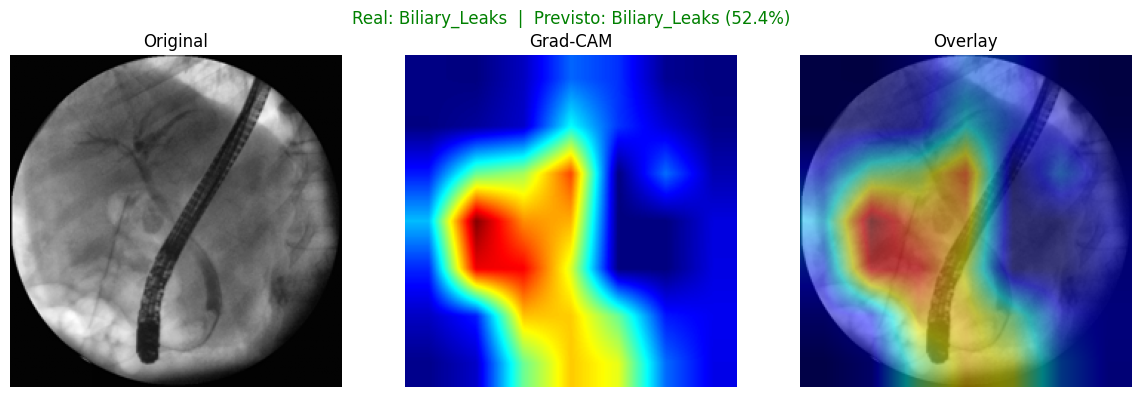
\includegraphics[width=0.95\textwidth]{images/biliaryleaks-correct-grad-cam.png}
    \caption{Biliary Leaks $\rightarrow$ Biliary Leaks (52.4\%) --- correcta.}
  \end{subfigure}\par\smallskip
  \begin{subfigure}{\textwidth}
    \centering
    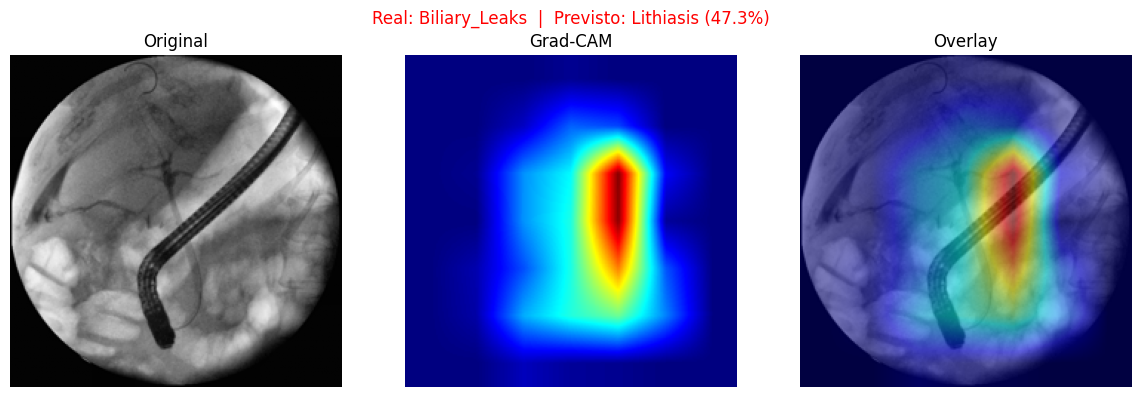
\includegraphics[width=0.95\textwidth]{images/biliaryleaks-wrong-grad-cam.png}
    \caption{Biliary Leaks $\rightarrow$ Lithiasis (47.3\%) --- incorrecta: heatmap activa o
      ducto principal, região morfologicamente semelhante a cálculos.}
  \end{subfigure}
  \caption{Grad-CAM --- Biliary Leaks (dois exemplos do conjunto de teste).}
  \label{fig:gradcam_bl}
\end{figure}

\begin{figure}[H]
  \centering
  \begin{subfigure}{\textwidth}
    \centering
    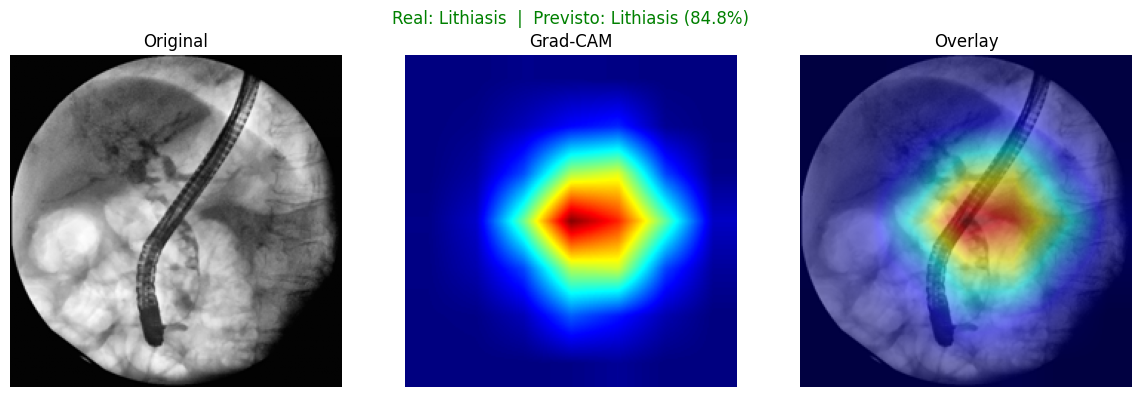
\includegraphics[width=0.95\textwidth]{images/lithiasis-correct-grad-cam.png}
    \caption{Lithiasis $\rightarrow$ Lithiasis (84.8\%) --- correcta: activação concentrada
      na zona de deposição de cálculos, com alta confiança.}
  \end{subfigure}
  \caption{Grad-CAM --- Lithiasis (exemplo de classificação correcta).}
  \label{fig:gradcam_li}
\end{figure}

\begin{figure}[H]
  \centering
  \begin{subfigure}{\textwidth}
    \centering
    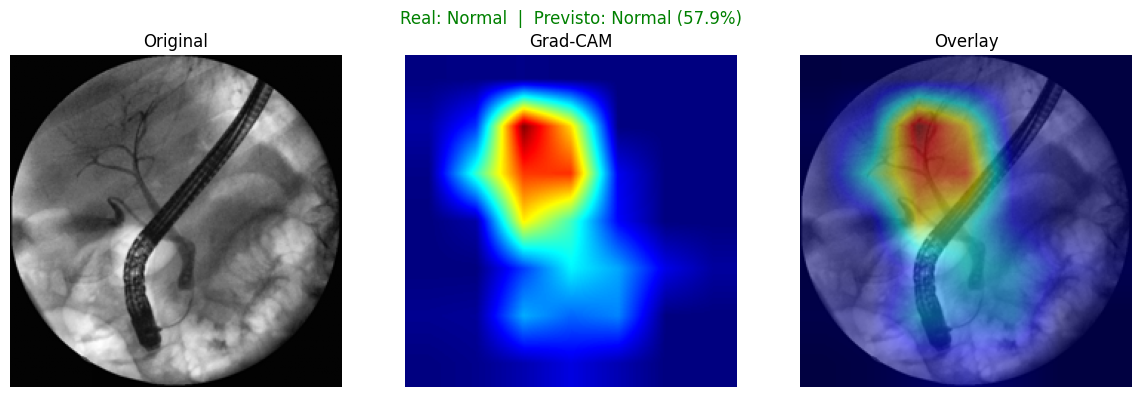
\includegraphics[width=0.95\textwidth]{images/normal-correct-grad-cam.png}
    \caption{Normal $\rightarrow$ Normal (57.9\%) --- correcta: heatmap difuso,
      sem foco em nenhuma região patológica.}
  \end{subfigure}\par\smallskip
  \begin{subfigure}{\textwidth}
    \centering
    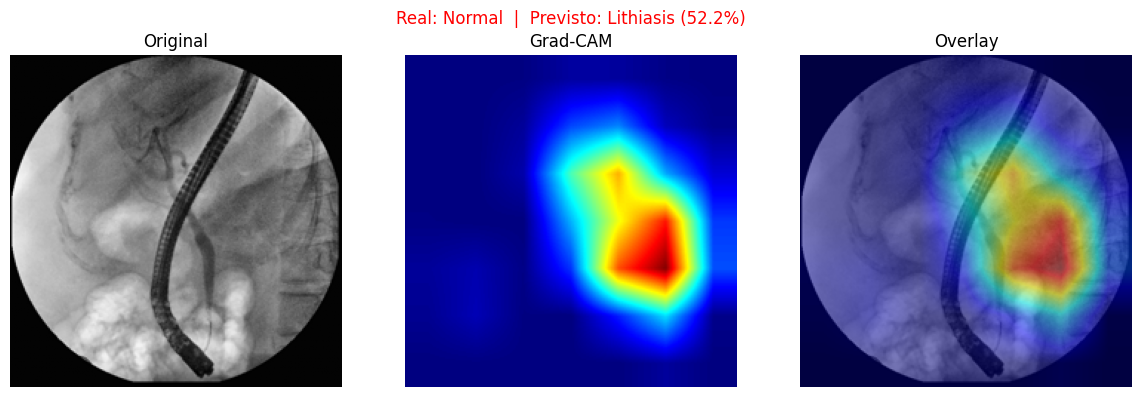
\includegraphics[width=0.95\textwidth]{images/normal-wrong-grad-cam.png}
    \caption{Normal $\rightarrow$ Lithiasis (52.2\%) --- incorrecta: o modelo activa uma
      região periférica semelhante à morfologia de cálculos.}
  \end{subfigure}
  \caption{Grad-CAM --- Normal (dois exemplos do conjunto de teste).}
  \label{fig:gradcam_no}
\end{figure}

\begin{figure}[H]
  \centering
  \begin{subfigure}{\textwidth}
    \centering
    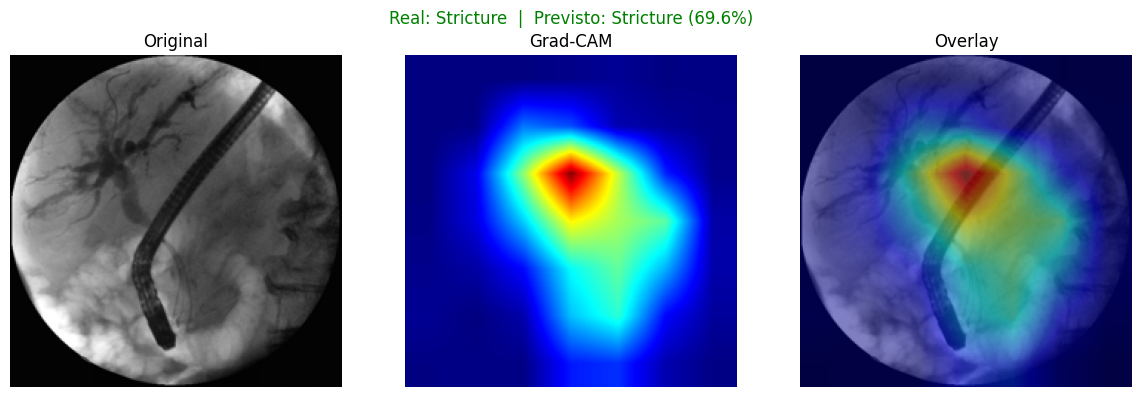
\includegraphics[width=0.95\textwidth]{images/stricture-correct-grad-cam.png}
    \caption{Stricture $\rightarrow$ Stricture (69.6\%) --- correcta: activação localizada
      na zona de estenose do ducto biliar.}
  \end{subfigure}\par\smallskip
  \begin{subfigure}{\textwidth}
    \centering
    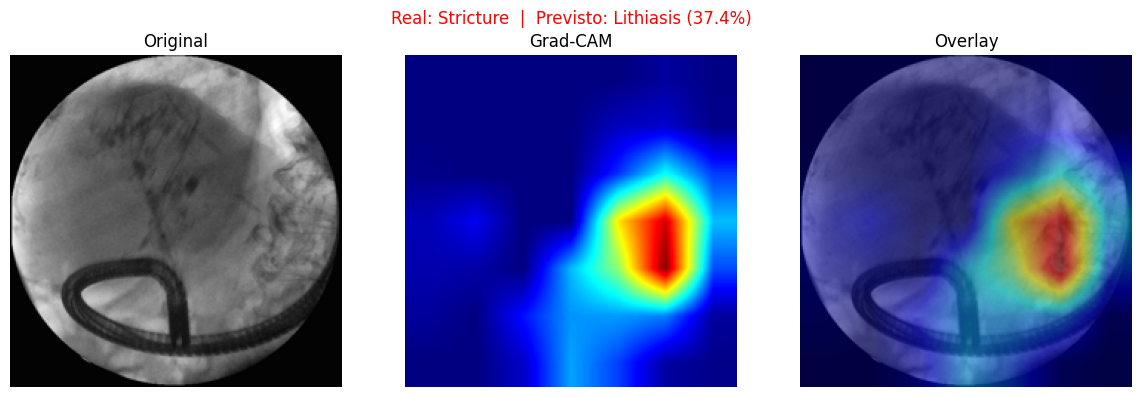
\includegraphics[width=0.95\textwidth]{images/stricture-wrong-grad-cam.png}
    \caption{Stricture $\rightarrow$ Lithiasis (37.4\%) --- incorrecta: heatmap activa
      uma estrutura tubular que o modelo interpreta como presença de cálculo,
      confirmando a confusão sistemática Stricture/Lithiasis.}
  \end{subfigure}
  \caption{Grad-CAM --- Stricture (dois exemplos do conjunto de teste).}
  \label{fig:gradcam_st}
\end{figure}

\section{Abordagem Ensemble}
Foi implementado um ensemble por soft voting entre DenseNet121 e
EfficientNet-B7:
\begin{equation}
P_{\text{ensemble}}(c\mid x) = \frac{1}{M}\sum_{m=1}^{M} P_m(c\mid x)
\end{equation}
Resultados preliminares com modelos base indicaram melhoria ligeira face aos
modelos isolados (F1 macro superior a 0.55). A combinação de versões mais
fortes (DenseNet121 com EfficientNet-B7 melhorada) mantém-se como direção de
continuação.

\section{Síntese e Conclusões}

\subsection{Ranking Final}
\begin{table}[ht]
\caption{Ranking final das arquiteturas.}
\label{tab:ranking}
\centering
\begin{tabular}{lccc}
\hline
Pos. & Arquitetura & F1 Macro & Accuracy \\
\hline
1 & DenseNet121 & \textbf{0.7076} & \textbf{0.7266} \\
2 & ResNet50 & \textbf{0.6647} & \textbf{0.7041} \\
3 & EfficientNet-B7 & \(\sim\)0.556 & \(\sim\)0.633 \\
4 & MobileNetV2 & \(\sim\)0.556 & \(\sim\)0.620 \\
\hline
\end{tabular}
\end{table}

\subsection{Conclusão Principal}
O tratamento explícito do desequilíbrio de classes foi o fator mais
determinante no desempenho final. A DenseNet121 combinou de forma mais eficaz
Focal Loss, class weighting, Mixup e TTA, alcançando F1 macro = 0.7076
(+16.3\,pp face ao baseline interno, v0). O gap de 3.0\,pp face à baseline
publicada~\cite{martins2025} (F1\,=\,0.738) indica que superar esse valor
requereria dados adicionais para Biliary Leaks ou arquiteturas de
atenção espacial (e.g.\ Vision Transformers), não exploradas neste trabalho.

\subsection{Trabalho Futuro}
As principais direções futuras são: (i) reforço de recall em Biliary Leaks com
amostragem ponderada e síntese de dados, (ii) validação cruzada estratificada
para estimativa robusta da variância, e (iii) ensemble entre os dois melhores
modelos individuais (DenseNet121 + ResNet50).

\begin{thebibliography}{10}
\bibitem{martins2025}
Martins, M.C. et al.: Curated endoscopic retrograde cholangiopancreatography
images dataset (MIQR-CC). Figshare (2025).
\url{https://doi.org/10.6084/m9.figshare.31079236}

\bibitem{he2016}
He, K., Zhang, X., Ren, S., Sun, J.: Deep residual learning for image
recognition. In: CVPR (2016)

\bibitem{huang2017}
Huang, G., Liu, Z., Van Der Maaten, L., Weinberger, K.Q.: Densely connected
convolutional networks. In: CVPR (2017)

\bibitem{lin2017}
Lin, T.-Y., Goyal, P., Girshick, R., He, K., Dollár, P.: Focal loss for dense
object detection. In: ICCV (2017)

\bibitem{pizer1987}
Pizer, S.M. et al.: Adaptive histogram equalization and its variations. CVGIP
(1987)

\bibitem{sandler2018}
Sandler, M., Howard, A., Zhu, M., Zhmoginov, A., Chen, L.-C.: MobileNetV2:
Inverted residuals and linear bottlenecks. In: CVPR (2018)

\bibitem{selvaraju2017}
Selvaraju, R.R. et al.: Grad-CAM: Visual explanations from deep networks. In:
ICCV (2017)

\bibitem{tajbakhsh2016}
Tajbakhsh, N. et al.: Convolutional neural networks for medical image analysis.
IEEE Transactions on Medical Imaging (2016)

\bibitem{tan2019}
Tan, M., Le, Q.: EfficientNet: Rethinking model scaling for convolutional
neural networks. In: ICML (2019)

\bibitem{zhang2018}
Zhang, H., Cissé, M., Dauphin, Y.N., Lopez-Paz, D.: Mixup: Beyond empirical
risk minimization. In: ICLR (2018)
\end{thebibliography}
\end{document}
